\section{Durchführung}
\label{sec:Durchführung}
\begin{figure}[H]
  \centering
  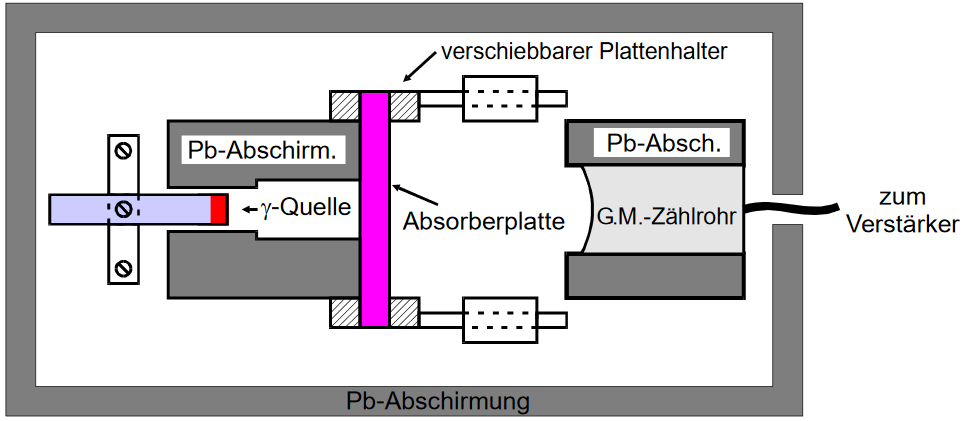
\includegraphics[height=6cm]{Aufbau.PNG}
  \caption{Aufbau der verwendeten Messapparatur. \cite{sample}}
  \label{fig:aufbau}
\end{figure}

Mit einer Messapparatur entsprechend Abbildung \ref{fig:aufbau} wird zu Beginn des
Versuchs der Nulleffekt gemessen. Dabei wird entsprechend noch keine $\gamma$-Quelle eingebaut,
sondern es wird über einen hinreichend langen Zeitraum (900 Sekunden) die Zählrate ohne
jeglichen Einfluss eines extra eingebauten Strahlers gemessen.

Anschließend wird dann eine Quelle eingebaut. Nun wird bei unterschiedlichen Dicken
der Absorberplatte die Zählrate über einen entsprechend langen Zeitraum (je dicker die
Platte, desto länger der Zeitraum) gemessen.

Eine analoge Messung wird anschließend auch für eine $\beta$-Quelle durchgeführt.
